\section{Antecedentes: modelo Mamba}

\label{sec:background}

El modelo Mamba (también conocido como Selective Scan Structured State Space o S6)~\cite{gu2023mamba} es un modelo sequence-to-sequence introducido recientemente que ofrece ventajas claras frente a enfoques existentes como convolutional networks (CNNs), recurrent networks (RNNs) y modelos self-attention (Transformers). Los modelos tradicionales, como la convolución y la recurrencia, son eficientes computacionalmente, pero tienen dificultades para capturar dependencias de largo alcance dentro de las secuencias. En contraste, self-attention sobresale en el modelado de dependencias de largo alcance, pero con un costo computacional mucho mayor, que escala cuadráticamente con la longitud de la secuencia. El modelo S6 combina lo mejor de ambos mundos: tiene la capacidad de modelar dependencias de largo alcance en secuencias mientras mantiene eficiencia computacional, logrando costo computacional y uso de memoria lineales.


\begin{figure*}[t]
    \centering
    \vspace{-5mm}
    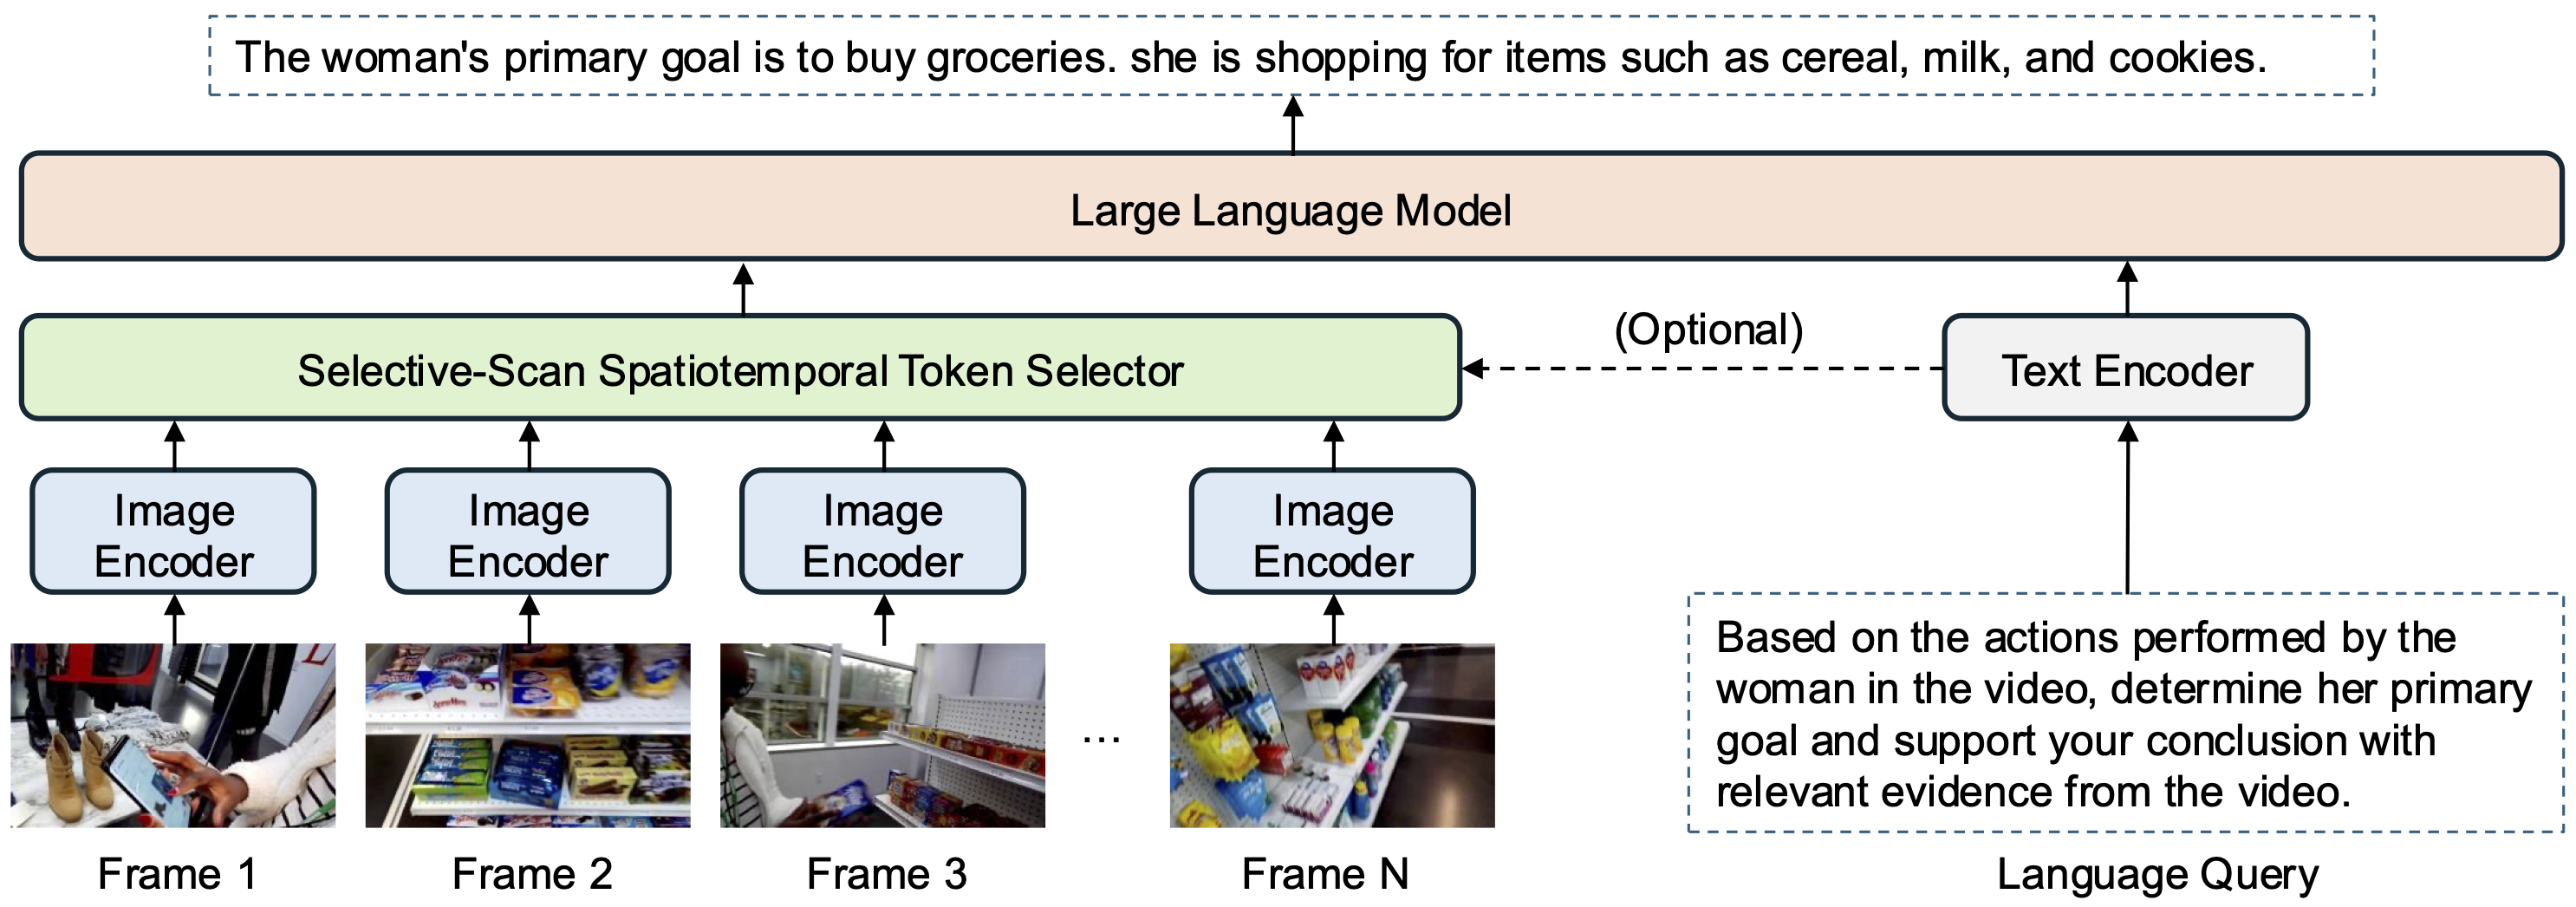
\includegraphics[width=\textwidth]
    {figures/model.png}
    \vspace{-7mm}
    \caption{\small{Nuestro modelo propuesto \model utiliza un Spatiotemporal Token Selector basado en Mamba para seleccionar una cantidad reducida de tokens salientes a partir de una larga secuencia de características extraídas mediante un pretrained image encoder. La selección de tokens puede condicionarse opcionalmente usando la consulta textual para identificar las características más informativas para responder una pregunta dada. Finalmente, los tokens seleccionados y transformados se envían a un large language model junto con una versión tokenizada de la pregunta de entrada para generar la respuesta.}}
    \vspace{-5mm}
\label{fig:model}
\end{figure*}


Teóricamente, el State-Space Model (SSM) representa un sistema continuo e invariante en el tiempo que mapea una señal de entrada $x(t) \in \mathbb{R}^L$ a una salida $y(t) \in \mathbb{R}^M$ a través de un estado oculto $h(t) \in \mathbb{R}^N$. Matemáticamente, los SSMs pueden describirse mediante un conjunto de ecuaciones diferenciales ordinarias lineales (ODEs):
\begin{equation}
    \begin{aligned}
    \label{eq:ssm}
    h'(t) &= \mathbf{A}h(t) + \mathbf{B}x(t), \\
    y(t) &= \mathbf{C}h(t) +  \mathbf{D}h(t).
    \end{aligned}
\end{equation}
Aquí, $ \mathbf{A} \in \mathbb{R}^{N \times N}$ representa la matriz de estado del sistema, $ \mathbf{B} \in \mathbb{R}^{N}$ y $ \mathbf{C} \in \mathbb{R}^{N}$ son matrices de proyección, y $ \mathbf{D} \in \mathbb{R}^1$ es la skip connection para un tamaño de estado $N$.

Para aplicar SSMs a datos del mundo real, la ODE continua~\eqref{eq:ssm} se discretiza primero usando la siguiente ecuación:
\begin{equation}
\begin{aligned}
\label{eq:discrete_ssm}
h_t &= \mathbf{\overline{A}}h_{k-1} + \mathbf{\overline{B}}x_{k}, \\
y_t &= \mathbf{C}h_k + \mathbf{D}x_k.
\end{aligned}
\end{equation}

Usando esta formulación, se ha propuesto una implementación eficiente de SSM llamada Structured State Space (S4)~\cite{gu2022efficiently}. S4 representa la matriz de estado $A$ como \textit{diagonal and low-rank}, lo que facilita un cómputo eficiente.

El modelo S4 es un sistema Linear Time-Invariant (LTI) con parámetros que permanecen constantes e independientes de la entrada. Esto puede ser subóptimo, especialmente para modelar dependencias de largo plazo en una secuencia que contiene información redundante y poco importante. Un trabajo reciente~\cite{gu2023mamba} propone Selective Scan State Space (S6) para desarrollar Mamba LLM~\cite{gu2023mamba}. En S6, las matrices $\mathbf{\overline{B}}$, $ \mathbf{C}$ y $\mathbf{\Delta}$ pasan a depender de la entrada y se derivan del input $x$ usando capas lineales.
\begin{equation}
\begin{aligned}
   \mathbf{B} = \text{Linear}_N(x)\\
   \mathbf{C} = \text{Linear}_N(x)
\end{aligned}
\end{equation}
Este enfoque selective-scan permite que los parámetros interactúen dinámicamente con la entrada a lo largo de la secuencia, posibilitando que el modelo retenga información importante y filtre datos redundantes. Como resultado, los modelos S6 se adaptan mejor a aplicaciones que requieren compresión eficiente de información, como la nuestra.
